\chapter{Resultados e Avaliação} \label{ch:evaluation}

A avaliação dos resultados foi realizada no Parque Computacional de Alto 
Desempenho (PCAD) da UFRGS. Os experimentos ocorreram nos nós de 
computação draco, sua configuração é mostrada na Tabela \ref{tab:draco_config}.

\begin{table}[H]
\centering
\begin{tabular}{l l} \toprule
\textbf{Parâmetro}  &  \textbf{Configuração} \\ 
\midrule
Processador     & 2 x Intel Xeon E5-2630 (Q1'12) Sandy Bridge, 2,5 GHz  
\\
Número de Núcleos    & 16 núcleos (8 por CPU)  \\
Memória       & 64 GB DDR3 RAM   \\
\end{tabular}
\caption{Configurações dos nós draco.}
\label{tab:draco_config}
\end{table}

A carga de trabalho dos experimentos já no formato CSV (entrada para a fase de 
pré-processamento no StarVZ), tinha um somatório de 12 GB. Ela consiste em 
rastros de execução de uma aplicação cholesky, e foi escolhida pois era a maior
entrada que tínhamos no momento. O tamanho de cada um dos arquivos pode ser 
visualizado na Tabela \ref{tab:input_sz}.

\begin{table}[H]
\centering
\begin{tabular}{l c} \toprule
\textbf{Arquivo}  &  \textbf{Tamanho} \\ 
\midrule
state.csv	& 6.8 GB \\
variables.csv  	& 2.5 GB \\
link.csv       	& 304 MB \\
dag.csv        	& 270 MB \\
entities.csv	& 73 KB \\
events.csv	& 1.8 GB \\
\textbf{Total}  & 12 GB  \\
\end{tabular}
\caption{Detalhamento da carga de trabalho.}
\label{tab:input_sz}
\end{table}

Durante a implementação, optou-se por manter o processamento do arquivo entities 
no formato sequencial pois esse arquivo armazena apenas informações de 
plataforma e por isso, costuma não passar da ordem de tamanho de KB. Podemos 
observar que isso se confirma nessa carga de trabalho.

Foram executados testes com um, dois e três nós. Para os distribuídos, 
armazenou-se os dados no HDFS, mas por facilidade de análise ao invés de 
utilizar o YARN como gerenciador de cluster utilizou-se o próprio Spark pois 
seus logs eram mais claros. Isso evidencia a flexibilidade que a engine Spark 
fornece pois, com um simples parâmetro, muda-se quem faz a gerência dos 
recursos ao executar a aplicação. 

A instância do Mestre Spark foi executada em um nó, junto com uma instância de 
Trabalhador, devido a quantidade de recursos presentes em uma máquina. Nas 
demais apenas o Trabalhador foi executado. As configurações que a Engine 
instânciou no ambiente por padrão podem ser visualizadas na tabela 
\ref{tab:spark_def_config}. Com 2 nós, o ambiente como um todo contou com 32 
executores enquanto com 3 nós, foram utilizados 45. Como simplesmente 
utilizou-se os valores padrão, é possível existir configurações que otimizam a 
performance da aplicação.

\begin{table}[H]
\centering
\begin{tabular}{c c c c} \toprule
\textbf{Número de nós}  &  \textbf{Executores por Nó} & \textbf{Cores por 
Executor} & \textbf{Memória por Executor} \\ 
\midrule
2	& 16 & 2 & 3 GB\\
3	& 15 & 2 & 4 GB\\
\end{tabular}
\caption{Ambiente instânciado pelo Spark.}
\label{tab:spark_def_config}
\end{table}

Sobre a metodologia dos testes, cada um teve 30 execuções. Houve falha em um 
teste distribuído de cada configuração, para estes, ficamos com 29 resultados 
apenas. O a média do tempo total de execução de cada uma das configurações pode 
ser visualizado na Figura \ref{fig:total_full}. Os desvios padrão das execuções 
pode ser visualizado no topo de cada barra. 

\begin{figure}[ht]
\centerline{
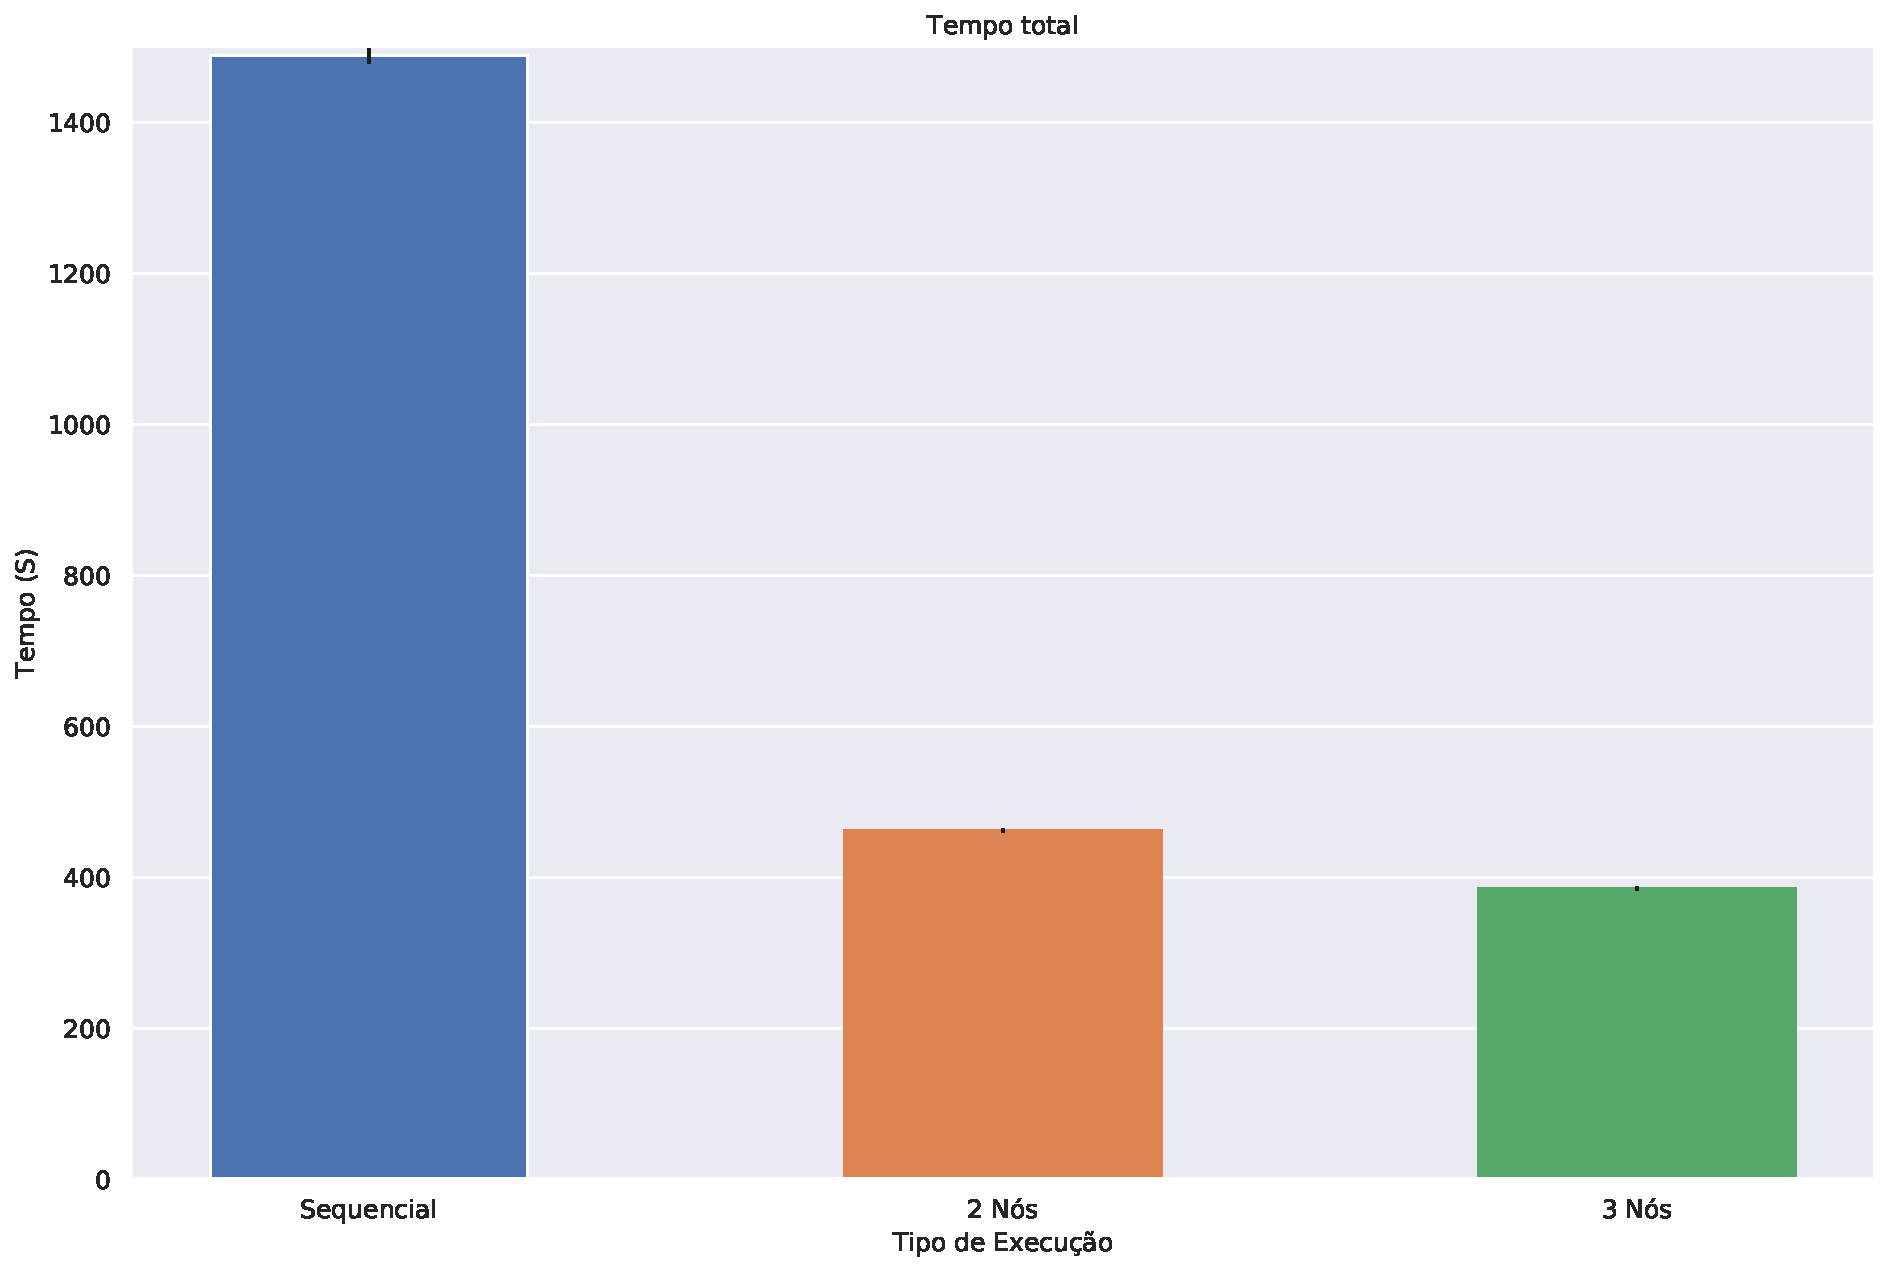
\includegraphics[width=0.8\textwidth]{./img/total.pdf}}
 \caption{Tempo total de execução da aplicação.}
 \label{fig:total_full}
\end{figure}





\begin{figure}[ht]
\centerline{
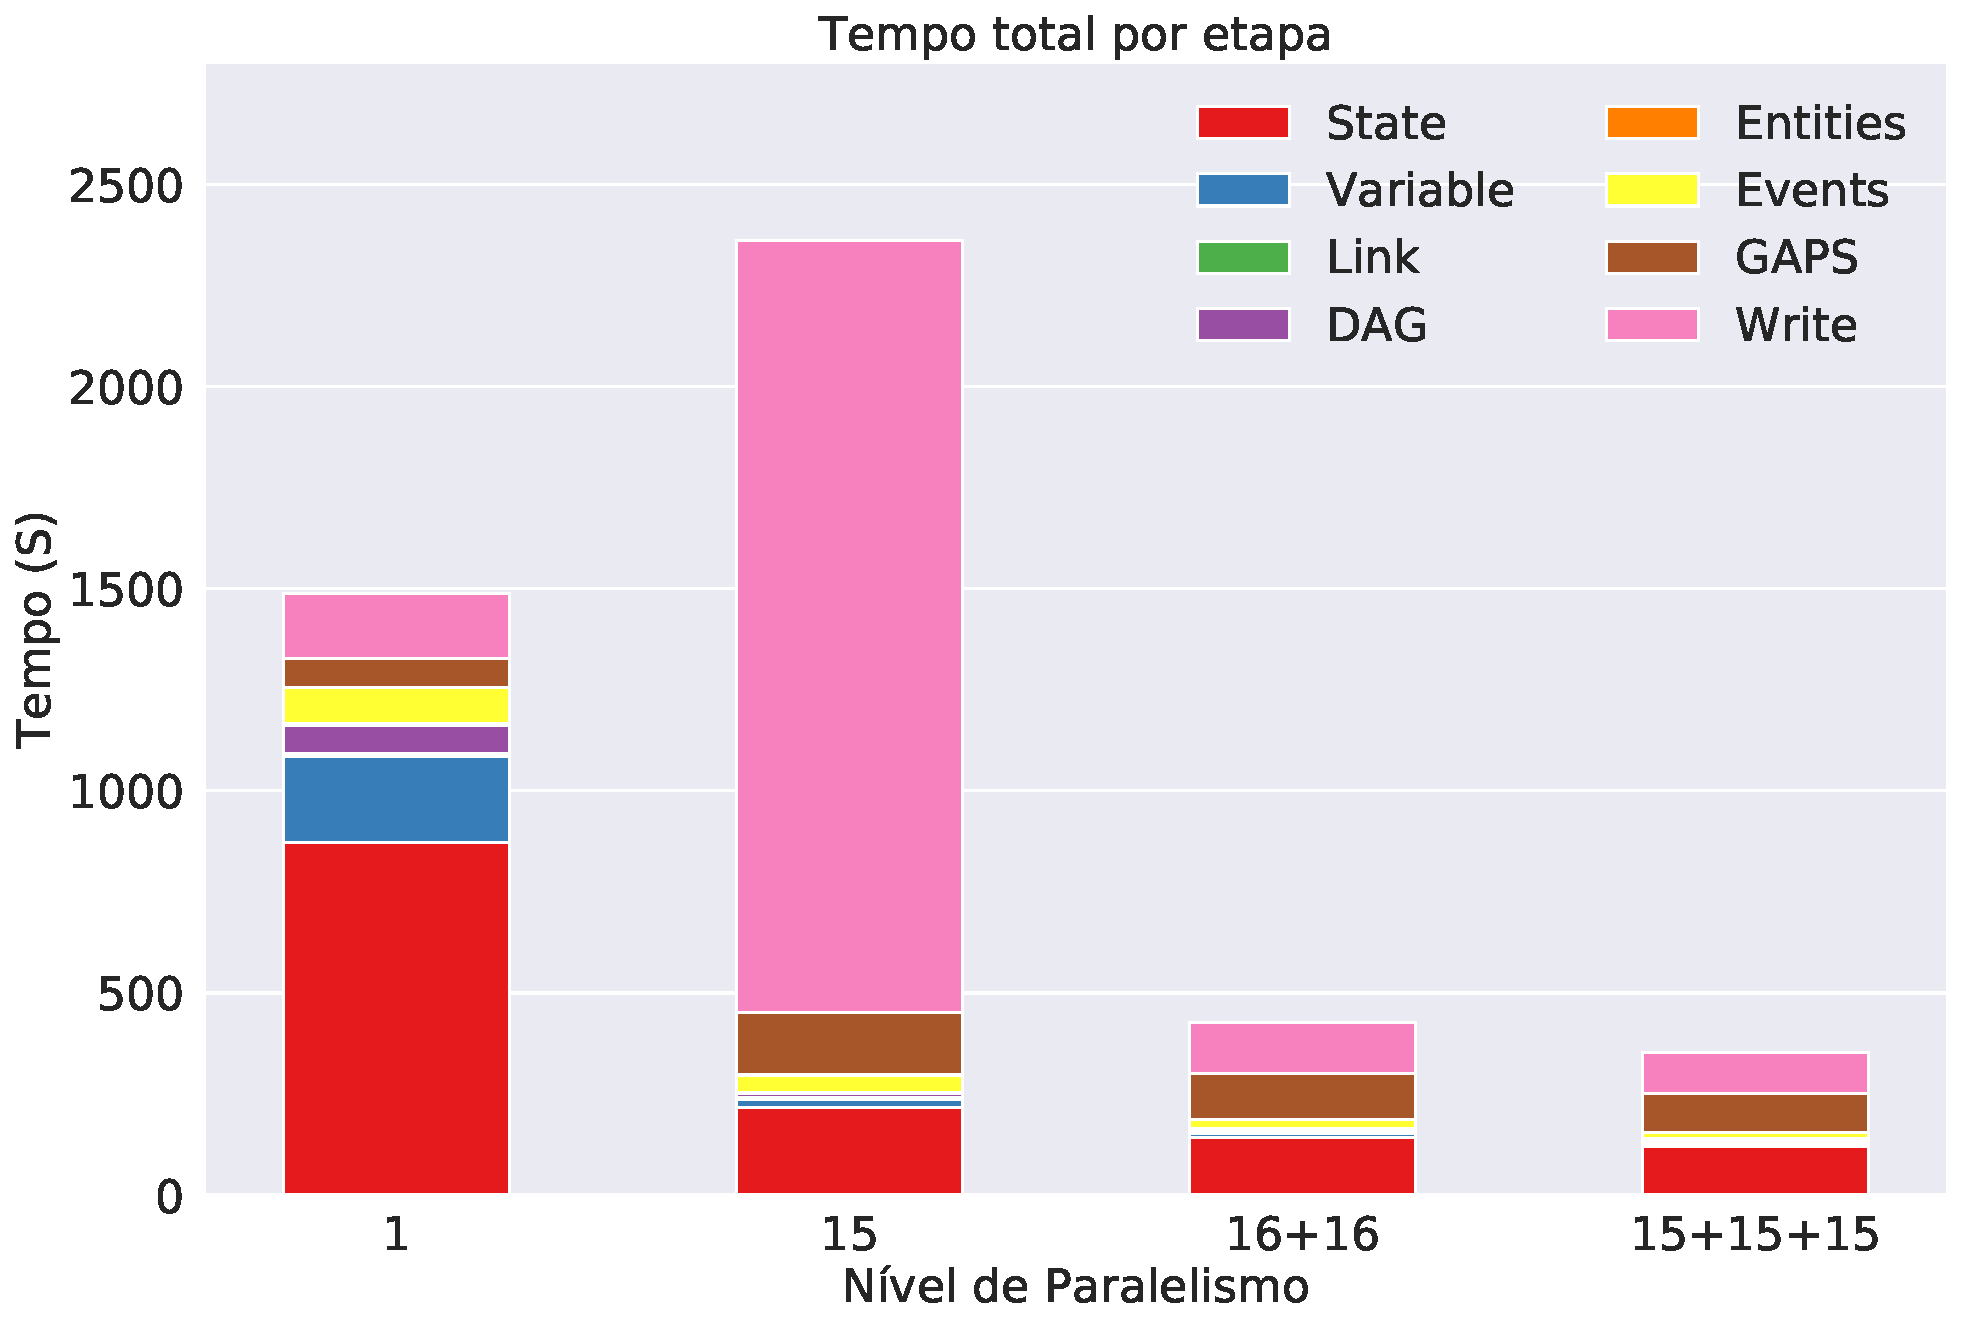
\includegraphics[width=0.8\textwidth]{./img/total_step.pdf}}
 \caption{Tempos por tipo de execução, segmentados por etapas.}
 \label{fig:total_step}
\end{figure}

